
\documentclass[9pt]{beamer}

\usepackage[latin1]{inputenc}
\usepackage{colortbl}
\usepackage[english]{babel}

\newcommand{\myblue} [1] {{\color{blue}#1}}
\newcommand{\newauthor}[4]{
  \parbox{0.26\textwidth}{
    \texorpdfstring
      {
        \centering
        #1 \\
        \myblue{{\href{#2}{\texttt{#3}}}} \\
        #4 \\
      }
      {#1}
  }
}


% for code colouring
\usepackage{minted}


% beamer template
\beamertemplatetransparentcovereddynamic
\usetheme{default}

\hypersetup{%
  pdftitle={Error Propagation in Go},%
   pdfauthor={Frank Sun},%
%
}

\title[Error Propagation in Go]{Error Propagation in Go}
\author[Frank Sun]{
 \parbox{0.26\textwidth}{
	\texorpdfstring
	  {
		\centering
 		Frank Sun \\
 		Golang Developer \\
 		\myblue{\href{mailto:elitegoblinrb@gmail.com}{\texttt{elitegoblinrb@gmail.com}}} \\
 		\myblue{\href{http://elitegoblin.github.io}{\texttt{http://elitegoblin.github.io}}} \\
 	  }
	{Frank Sun}
}
 }

\date{2019-04-24}

\begin{document}

\frame{\titlepage
}

\part<presentation>{Main Talk}

\section[slides]{slides}

\begin{frame}[fragile]
\frametitle{Roadmap}


\begin{itemize}
\item Customers of error handling(Why we need it)
\item Caller perspective: API error response
\item Developer perspective: how error propgate, structure error logs
\end{itemize}


\end{frame}

\begin{frame}[fragile]
\frametitle{Scope}


In scope: 


\begin{itemize}
\item Error passing between services
\item Error propagation inside a service/process: between functions, go packages, go routines
\end{itemize}

Out of scope: 


\begin{itemize}
\item Panic handle
\end{itemize}


\end{frame}

\begin{frame}[fragile]
\frametitle{Customers of error handling}


\begin{itemize}
\item Caller of our API
\item Deveoper of service(Gophers)
\end{itemize}


\end{frame}

\begin{frame}[fragile]
\frametitle{Caller perspective: API error response}


Error response must be helpful on caller's perspective


\begin{itemize}
\item HTTP Status Code
\item Internal Reference Code
\item Human readable messages
\end{itemize}


\end{frame}

\begin{frame}[fragile]
\frametitle{HTTP Status Code}


\begin{itemize}
\item 1XX – Informational
\item 2XX – Success
\item 3XX – Redirection
\item 4XX – Client Error: 404 Not Found, 429 Too many Requests
\item 5XX – Server Error: 502 Bad Gateway, 503 Service Unavailable
\end{itemize}

Some company use Http 200 for almost all response(even error occured), use other reference code to indicate error



\end{frame}

\begin{frame}[fragile]
\frametitle{Internal Reference Code}


Business logic related error code, example: 


800001 means insufficient credits when user try to make a call



\end{frame}

\begin{frame}[fragile]
\frametitle{Human readable messages}


Should contains: 


\begin{itemize}
\item Cause
\item Summarized context
\item General solution for the error at hand
\end{itemize}


\end{frame}

\begin{frame}[fragile]
\frametitle{API error response example: }


A error response


\begin{minted}[]{json}
{
  "code": 404001,
  "message": "userId not found",
  "traceId": "business_wzfw_work-location_000001",
  "data": null
}

\end{minted}

A successful response


\begin{minted}[]{json}
{
  "code": 200,
  "message": "",
  "traceId": "business_wzfw_work-location_000001",
  "data": {
    "msisdn": "17321452140",
    "zipCode": 21,
    "provId": 831,
    "cityCode": 83101,
    "location": "31.14570,121.54082",
    "occurTime": "2017-05-23T09:52:07.000Z"
  }
}

\end{minted}


\end{frame}

\begin{frame}[fragile]
\frametitle{Developer perspective}


How error flow through inside the service  


Error flow should NOT be treated as second-class citizen as to control flow


Goals:


\begin{itemize}
\item Record whole error flow
\item Ability to retrieve it in log
\end{itemize}


\end{frame}

\begin{frame}[fragile]
\frametitle{Golang internal error support}


\begin{minted}[]{go}
// built-in interface type

type error interface {
        Error() string
}

package errors
// New returns an error that formats as the given text.
func New(text string) error {
	return &errorString{text}
}
// errorString is a trivial implementation of error.
type errorString struct {
	s string
}
func (e *errorString) Error() string {
	return e.s
}
package fmt
func Errorf(format string, a ...interface{}) error {
	return errors.New(Sprintf(format, a...))
}

\end{minted}


\end{frame}

\begin{frame}[fragile]
\frametitle{What we usually do}


\begin{minted}[]{go}
package midlevel

func Do() error{
	err := lowlevel.Execute(cmd)
	if err != nil {
		// long error msg string, need to consistent in every level, no call stack
	    return fmt.Errorf("get a error in midlevel Do: %s", err)
	    // sometimes we do: 
	    // lose context of root cause and error flow
	    return fmt.Errorf("get a error in midlevel Do")
	    // or
	    // lose context of midlevel
	    return err
	}
}

\end{minted}


\end{frame}

\begin{frame}[fragile]
\frametitle{Pain points}


No framework support, no standard way to pass the errors 


Missing context when passing errors



\end{frame}

\begin{frame}[fragile]
\frametitle{What we should do}


\begin{itemize}
\item Always pass error back to caller
\item Add context: error propagate chain, each node's stacktrace in chain
\item When passing error back to caller, hide(not remove) details, optional
\end{itemize}


\end{frame}

\begin{frame}[fragile]
\frametitle{Propagate error up in control flow}


Avoid swallowing error


\begin{figure}[h]
\begin{center}
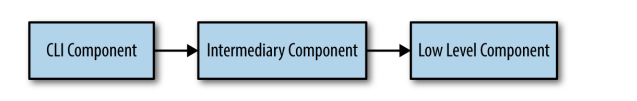
\includegraphics[width=10cm,height=1cm]{images/chain.png}
\end{center}

\end{figure}


\end{frame}

\begin{frame}[fragile]
\frametitle{Add Context using pkg/errors}


\begin{itemize}
\item Simple error handling primitives
\item 4300+ stars, one maintainer from Google Golang team
\item Recommended by author of Concurrency in Go
\end{itemize}


\end{frame}

\begin{frame}[fragile]
\frametitle{pkg/errors}


\begin{itemize}
\item New(message string) error
\item Errorf(format string, args ...interface\{\}) error
\item Wrapf(err error, message string,  args ...interface\{\}) error
\item Cause(err error) error
\end{itemize}


\end{frame}

\begin{frame}[fragile]
\frametitle{pkg/errors example: New, Errorf}


\begin{minted}[]{go}
import (
	"fmt"

	"github.com/pkg/errors"
)

func ExampleNew() {
	err := errors.New("whoops")
	fmt.Println(err)

	// Output: whoops
}

func ExampleNew_printf() {
	err := errors.New("whoops")
	fmt.Printf("%+v", err)

	// Example output:
	// whoops
	// github.com/pkg/errors_test.ExampleNew_printf
	//         /home/dfc/src/github.com/pkg/errors/example_test.go:17
	// testing.runExample
	// ...
}

\end{minted}


\end{frame}

\begin{frame}[fragile]
\frametitle{pkg/errors: New, Errorf}


\begin{itemize}
\item Leaf node of error tree
\item Should be closest to where error first occurs
\end{itemize}


\end{frame}

\begin{frame}[fragile]
\frametitle{pkg/errors: propagate error(relay)}


Wrap/Wrapf


\begin{minted}[]{go}
func ExampleWrap() {
	cause := errors.New("file not exist")
	err := errors.Wrap(cause, "can not write content")
	fmt.Println(err)

	// Output: can not write content: file not exist
}

\end{minted}


\end{frame}

\begin{frame}[fragile]
\frametitle{pkg/errors: show stack}


\begin{minted}[]{go}
func fn() error {
	e1 := errors.New("error")
	e2 := errors.Wrap(e1, "inner")
	e3 := errors.Wrap(e2, "middle")
	return errors.Wrap(e3, "outer")
}

\end{minted}


\end{frame}

\begin{frame}[fragile]
\frametitle{pkg/errors: show cause}


\begin{minted}[]{go}
func ExampleCause() {
	err := fn()
	fmt.Println(err)
	fmt.Println(errors.Cause(err))

	// Output: outer: middle: inner: error
	// error
}

\end{minted}


\end{frame}

\begin{frame}[fragile]
\frametitle{pkg/errors: show stack}


\begin{minted}[]{go}
func ExampleWrap_extended() {
	err := fn()
	fmt.Printf("%+v\n", err)
	// Example output:
	// error
    // _/home/frankie/git_repo/errors_test.fn
	//    /home/frankie/git_repo/errors/example_test.go:100
    // _/home/frankie/git_repo/errors_test.ExampleWrap_extended
	//    /home/frankie/git_repo/errors/example_test.go:116
	// ... more error stack
	// inner
	// ... inner's stack
	// middle
	// ... middle's stack
	// outter
	// ... outter's stack
}

\end{minted}


\end{frame}

\begin{frame}[fragile]
\frametitle{Passing errors between goroutines?}


Same, use error channel to pass error back to caller



\end{frame}

\begin{frame}[fragile]
\frametitle{Typed error?}


Sometimes we need: 


\begin{itemize}
\item Execute different code path by error returned
\item Check if wrapped error or raw error(should be seemed as code bug if we use pkg/errors)
\end{itemize}

We can define our own error type(struct)


\begin{minted}[]{go}
type MyError struct {
	error
}

func (err MyError) Error() string {
	return err.Error()
}

\end{minted}

Author of Concurrency in Go suggested: we should defined error type in package level, each package wrap/format error escaped from current package(My idea is that only necessary for large projects)



\end{frame}

\begin{frame}[fragile]
\frametitle{Go2 proposal about error handling}


Try/catch mechanism to make code clean and robust



\end{frame}

\begin{frame}[fragile]
\frametitle{Conclusion}


\begin{itemize}
\item API response we consider: add additional error code; summaried, human readable message; attach traceId
\item Pass error back to root caller who log it, avoid swallowing error
\item Use pkg/errors to replace errors package to add more context
\item Use typed error with care, bottom line is do not create wrong dependency between packages
\end{itemize}


\end{frame}

\begin{frame}[fragile]
\frametitle{Reference}


Chapter 5 Concurrency at scale, section Error Propagation, Concurrency in Go by Katherine Cox-Buday  


\myblue{\href{https://nordicapis.com/best-practices-api-error-handling/}{\texttt{Best Practices for API Error Handling}}}

\myblue{\href{https://tools.ietf.org/html/rfc7807}{\texttt{RFC 7807: Problem Details for HTTP APIs}}}

\myblue{\href{https://github.com/pkg/errors/blob/master/example_test.go}{\texttt{pkg/errors example}}}

\myblue{\href{https://go.googlesource.com/proposal/+/master/design/go2draft-error-handling-overview.md}{\texttt{Error Handling — Problem Overview}}}

\myblue{\href{https://dave.cheney.net/2016/04/27/dont-just-check-errors-handle-them-gracefully}{\texttt{Don’t just check errors, handle them gracefully}}}


\end{frame}

\end{document}
